\chapter{Protostellar Disks and Outflows: Observations}
\label{ch:disks_obs}

\marginnote{
\textbf{Suggested background reading:}
\begin{itemize}
\item \href{http://adsabs.harvard.edu/abs/2014prpl.conf..173L}{Li, Z.-Y., et al. 2014, in ``Protostars and Planets VI", ed.~H.~Beuther et al., pp.~173-194}, sections 1-2 \nocite{li14a}
\end{itemize}
\textbf{Suggested literature:}
\begin{itemize}
\item \href{http://adsabs.harvard.edu/abs/2012Natur.492...83T}{Tobin et al., 2012, \textit{Nature}, 492, 83} \nocite{tobin12a}
\end{itemize}
}

We now zoom in even further on the star formation process, and examine the dominant circumstellar structures found around young stars: accretion disks. We will spend two chapters on this subject. In the first we will discuss the observational phenomenology of disks, including the outflows they generate. There are a wide range of observational techniques for studying the properties of disks around young stars, and we will certainly not exhaust the list here. We will focus on a few of the most widely used methods, and develop an understanding of how they work and what we can learn from them.

\section{Observing Disks}

\subsection{Dust at Optical Wavelengths}

\begin{marginfigure}
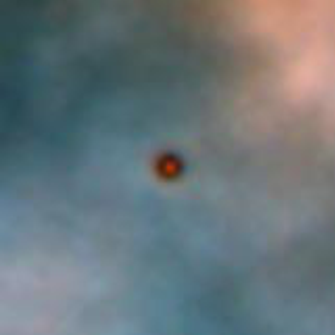
\includegraphics[width=\linewidth]{proplyds1}
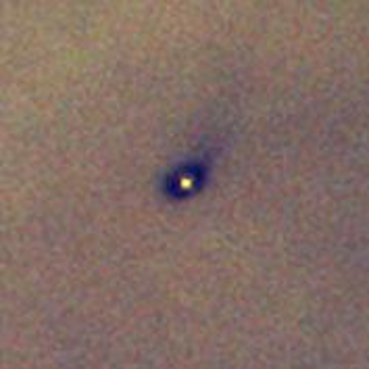
\includegraphics[width=\linewidth]{proplyds2}
%\includegraphics[width=\linewidth]{proplyds3}
\caption[Protostellar disks in absorption in the ONC]{
\label{fig:proplyds}
Two disks in the Orion Nebula seen in absorption against the nebula using \textit{HST}. Taken from \url{http://hubblesite.org/newscenter/archive/releases/1995/45/image/g/}.
}
\end{marginfigure}

The first idea that might occur to an astronomer who wants to study disks would be to work in the optical. The main challenge to that is that for the most part disks do not emit optical light, because they are too cool. This leaves only a couple of options in the optical. One is that we can detect the disk in scattered starlight. This is very hard, because the light is very faint, and the geometry has to be just right. Polarization can help in this case, since the scatter light will be polarized. There are a few examples of this.

The other possibility for the optical is to work in absorption. This requires a bright, extended background source against which the disk can be detected in silhouette. Fortunately, massive young stars produce H~\textsc{ii} regions, which are bright diffuse sources, and can provide a nice backlight for absorption work. The most spectacular examples of this technique are in the Orion Nebula, as illustrated in Figure \ref{fig:proplyds}.

In this case, since we are working in optical, we get excellent spatial resolution. The disks we see in this case are typically hundreds of AU in size. In such images we can also see very clearly that protostellar jets are launched perpendicular to the disks, confirmed the central role of disks in producing them, as we will discuss shortly.

While the optical offers spectacular pictures, its restriction to the cases where we have favorable geometry, a nice backlight, or some combination of the two limits its usefulness as a general tool for studying disks. A further complication is that optical only lets us study disks once their parent cores, which are optically thick at optical wavelengths, have dissipated. This limits optical techniques to studying the later stages of disk evolution.


\subsection{Dust Emission in the Infrared and Sub-mm}

A much more broadly used technique is to detect the dust in a disk in the infrared or sub-mm. As discussed in Chapter \ref{ch:obsstars}, young stars often show significantly more IR and sub-mm emission that would be expected from a bare stellar photosphere. The natural candidate for producing this emission is warm dust grains near the star. The fact that we see the stellar photosphere at all, and that it is not hugely reddened, implies that the grains cannot be in any sort of shell or spherical distribution. A disk is the natural candidate geometry.

\begin{marginfigure}
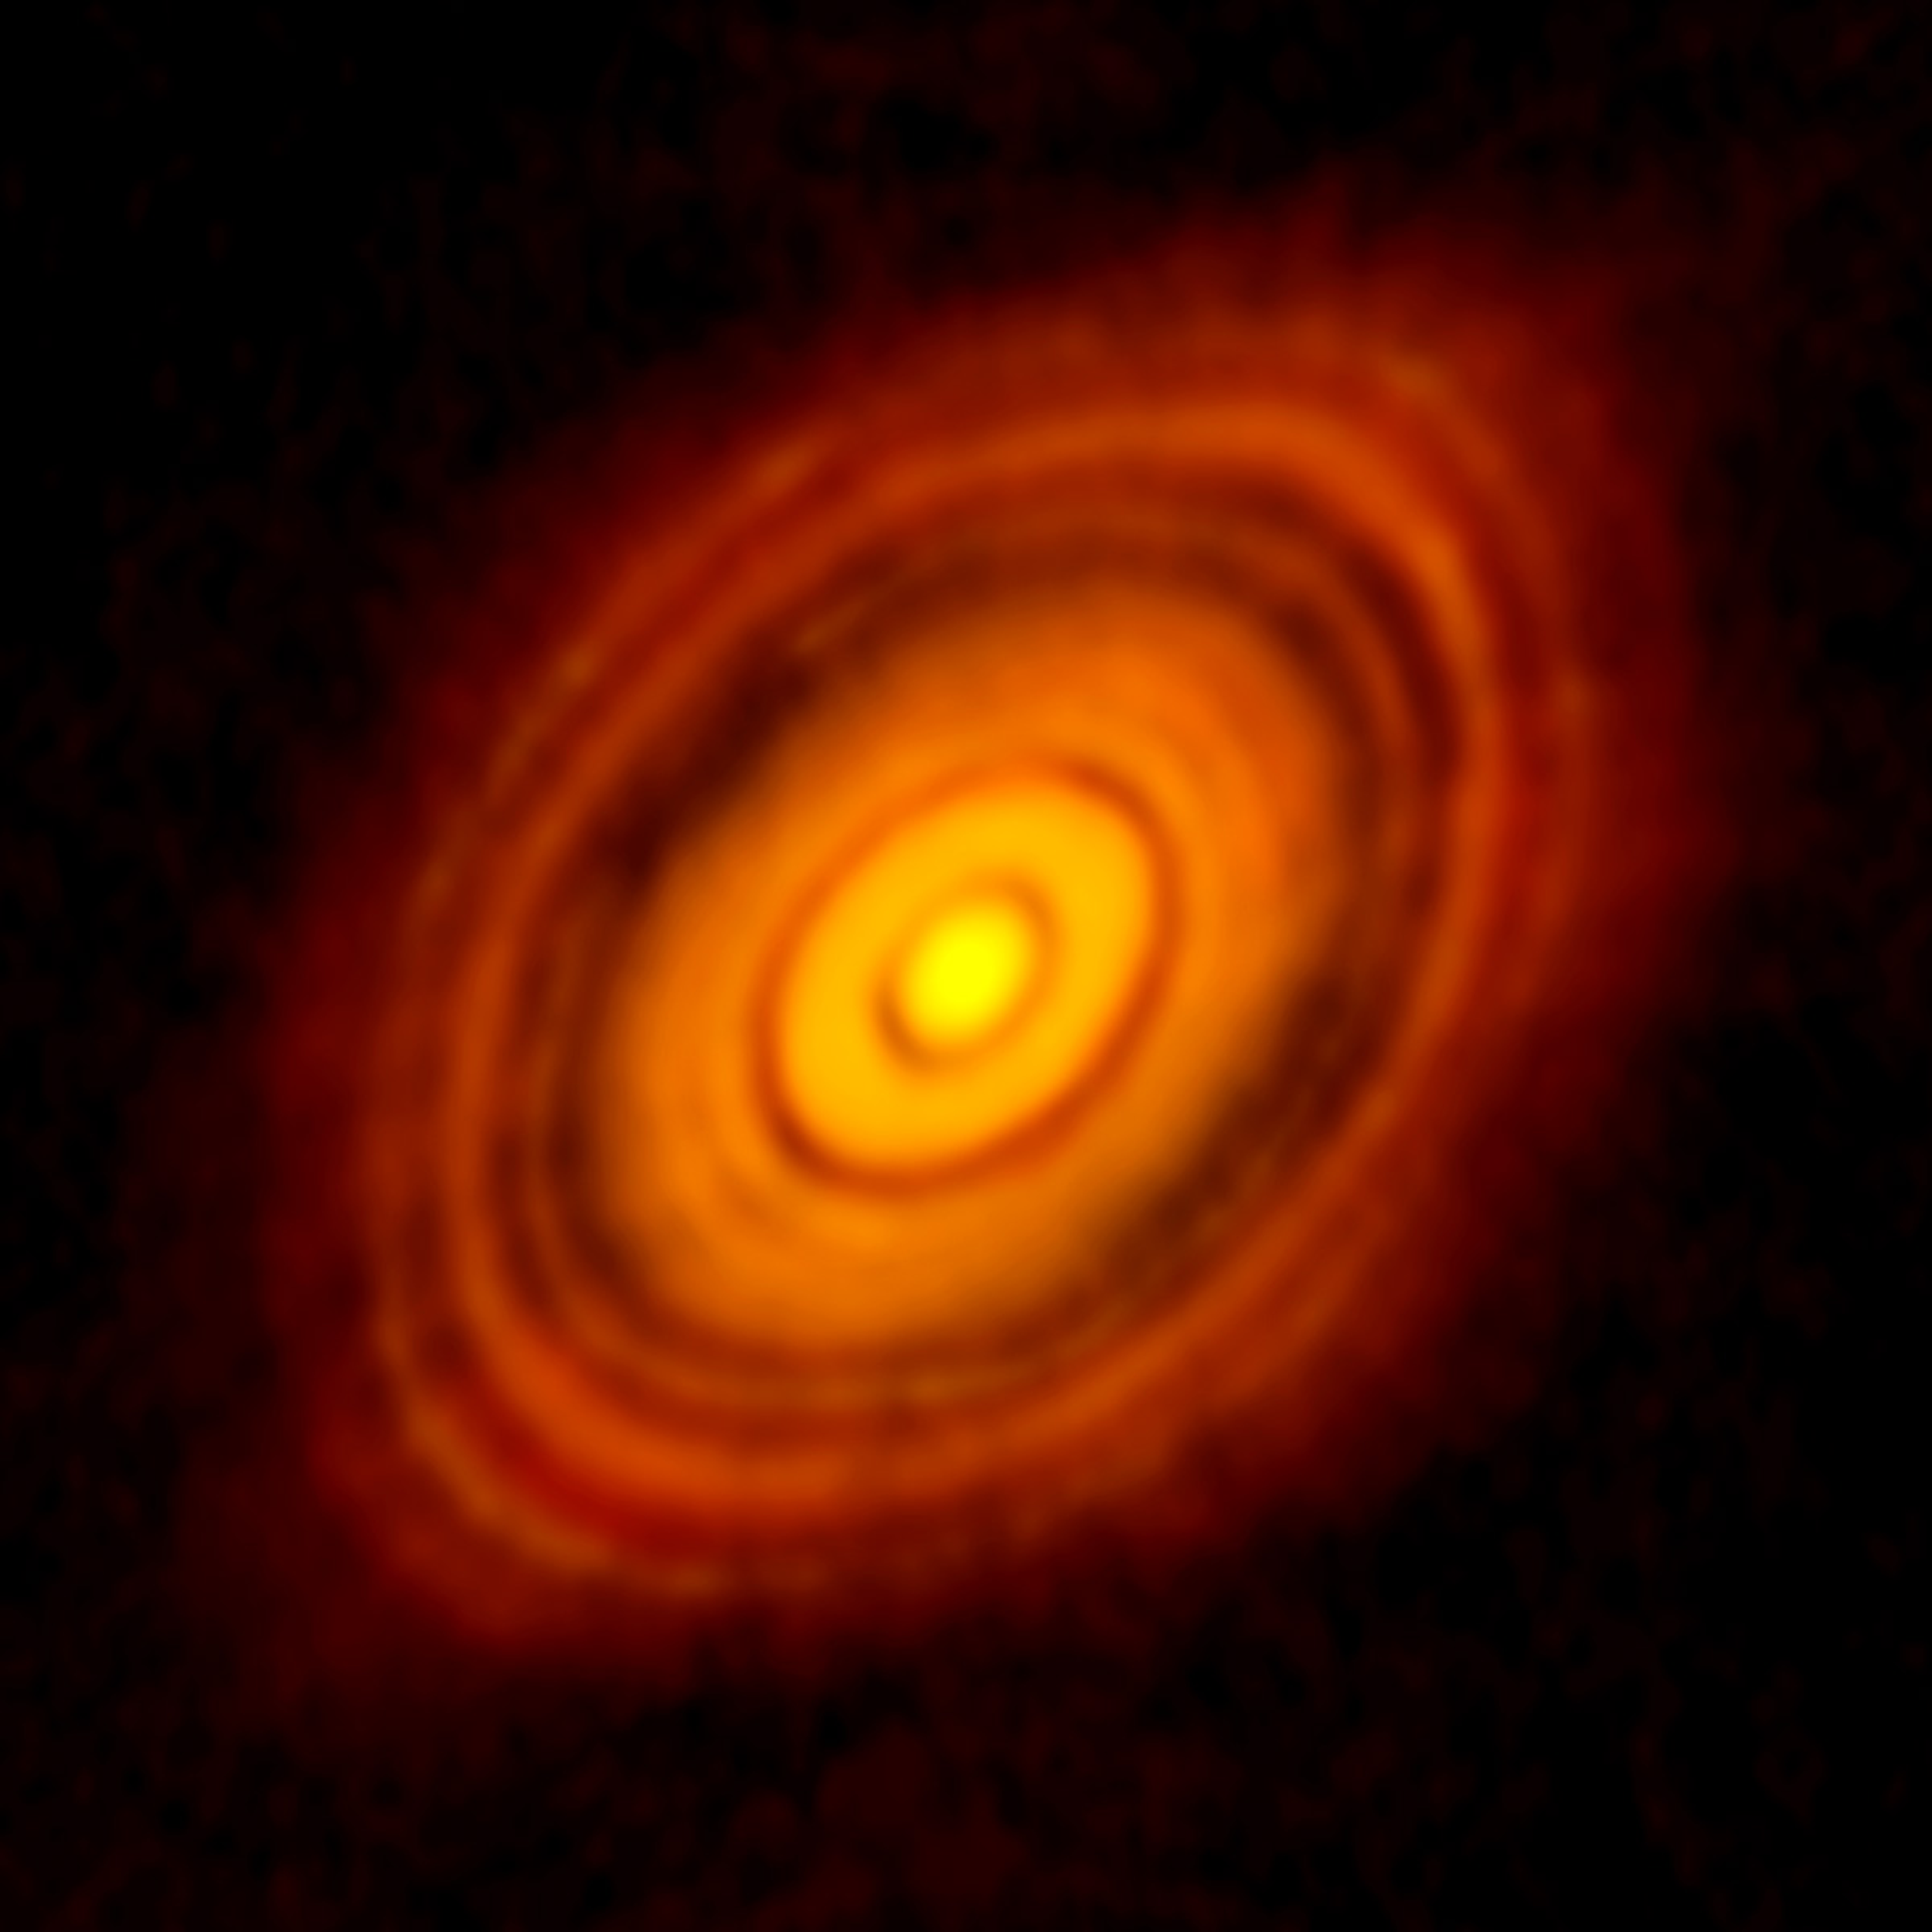
\includegraphics[width=\linewidth]{HLTau_nrao}
\caption[ALMA image of the disk around HL Tau]{
\label{fig:hltau_nrao}
An ALMA image of the disk around the young star HL Tau. The image shows dust continuum emission. Image from \url{https://public.nrao.edu/static/pr/planet-formation-alma.html}.
}
\end{marginfigure}

In some cases we can spatially resolve a disk in IR or sub-mm observations (Figure \ref{fig:hltau_nrao}), and in some cases the disks are unresolved. In either case, in order to interpret these images, we need to think a bit about which parts of the disk we expect to see at which wavelengths. Consider a geometrically thin disk of material of surface density $\Sigma(\varpi)$ and temperature $T(\varpi)$ beginning at a radius $\varpi_0$ around the star and extending out to radius $\varpi_1$. The dust has opacity $\kappa_\lambda$ at wavelength $\lambda$. The entire disk is inclined relative to our line of sight at angle $\theta$. The flux we receive from the disk at wavelength $\lambda$ is
\begin{equation}
F_{\lambda} = \int I_{\lambda}\, d\Omega,
\end{equation}
where $I_{\lambda}$ is the intensity emitted by a portion of the disk at wavelength $\lambda$, and the integral goes over the solid angle $\Omega$ occupied by the disk.

To evaluate this, note the ring of material at radius $\varpi$ has an area $2\pi \varpi \,d\varpi$. It is inclined relative to the line of sight by $\theta$, however, so its projected area is $2\pi \varpi \cos\theta\, d\varpi$. The case $\theta=0$ corresponds to the ring being seen perfectly face-on, and the case $\theta=1$ corresponds to perfectly edge-on, and gives 0 in the limit of an infinitely thin disk. This is the projected area, and to covert this to a projected solid angle we divide by $D^2$, where $D$ is the distance to the disk. Thus the flux is
\begin{equation}
F_{\lambda} = \frac{2\pi \cos\theta}{D^2} \int_{\varpi_0}^{\varpi_1} I_\lambda(\varpi) \varpi\, d\varpi.
\end{equation}

To make further progress we must specify the intensity, which is a function of $\Sigma$ and $T$. The optical depth of the disk will be
\begin{equation}
\tau_{\lambda} = \frac{\kappa_{\lambda}\Sigma}{\cos\theta}
\end{equation}
Note that the inclination factor $\cos\theta$ appears on the bottom here, as it should: for $\theta=0$, face-on, we just get the ordinary surface density, but that gets boosted as we incline the disk. The intensity produced by a slab of material of uniform temperature $T$ and optical depth $\tau_{\lambda}$ is
\begin{equation}
I_{\lambda} = B_{\lambda}(T) \left(1-e^{-\tau_{\lambda}}\right),
\end{equation}
where $B_{\lambda}(T)$ is the Planck function. Plugging this in, we have
\begin{equation}
F_{\lambda} = \frac{2\pi \cos\theta}{D^2} \int_{\varpi_0}^{\varpi_1} B_{\lambda}(T) \left[1-\exp\left(-\frac{\kappa_{\lambda}\Sigma}{\cos\theta}\right)\right] \varpi\, d\varpi.
\end{equation}

For a given disk model it is clearly straightforward to evaluate this integral to obtain the emitted flux. However, the model is underspecified, in the sense that we are fitting only one function, $F_{\lambda}$, and we have two free-functions to use: $T(\varpi)$ and $\Sigma(\varpi)$. This is even if we assume that the opacity is known, which we will see is not a great assumption.

In order to deduce things like $\Sigma$ and $T$ we need to have a physical model of how the disk behaves, and to deduce either $\Sigma$, $T$, or a relationship between them in order to obtain strong constraints on either one from an observed SED. In general such models can be quite complicated, because the disk's temperature distribution depends on both internal heating via viscous dissipation, and external illumination due to the star. Problem set 4 contains a problem in whuch such a model is developed. Even without such a sophisticated model, however, it is possible to learn very interesting things simply from the behavior of the flux in certain limits.

\paragraph{The optically thick limit.}

First, suppose that the disk is optically thick at some wavelength, i.e.\ $\tau_{\lambda} = \kappa_{\lambda}\Sigma/\cos\theta \gg 1$. This is likely to be true for shorter (e.g.\ near-IR) wavelengths, where the opacity is high, and where most emission is coming form close to the star where the surface density is highest. In this case it is reasonable to set the exponential factor to 0, and we are simply left with the integral of the Planck function of the disk temperature over radius.

Note that in this limit $\Sigma$ drops out, which makes intuitive sense: if the disk is optically thick then we only get to see its surface, and adding or removing material beneath this surface won't change the amount of light we see. Substituting in the Planck function, in the optically thick case we now have
\begin{equation}
F_{\lambda} = \frac{4\pi\cos\theta}{D^2} \frac{hc^2}{\lambda^5} \int_{\varpi_0}^{\varpi_1} \frac{\varpi}{\exp[hc/(k_B T)]-1}\,d\varpi.
\end{equation}

If we further assume that the temperature varies with radius as a powerlaw, $T=T_0(\varpi/\varpi_0)^{-q}$, then we can evaluate the integral via the substitution
\begin{equation}
x=\left(\frac{hc}{\lambda k_B T_0}\right)^{1/q} \frac{\varpi}{\varpi_0},
\end{equation}
which gives
\begin{eqnarray}
F_{\lambda} & = & 
\frac{4\pi \cos\theta}{D^2} \frac{hc^2}{\lambda^5} \left(\frac{\varpi_0}{x_0}\right)^2 \int_{x_0}^{x_1} \frac{x}{\exp(x^q)-1}\,dx \\
& = & 
\frac{4\pi \cos\theta}{D^2} \frac{hc^2}{\lambda^5} \left(\frac{hc}{\lambda k_B \varpi_0^q T_0}\right)^{-2/q} \int_{x_0}^{x_1} \frac{x}{\exp(x^q)-1}\,dx,
\end{eqnarray}
and $x_0$ and $x_1$ are obtained by plugging $\varpi_0$ and $\varpi_1$ into the expression for $x$.

If we look at the part of the SED where emission is dominated neither by the inner edge of the disk nor the outer optically thin parts, which will be the case over most of the IR, then we can set $x_0\approx 0$ and $x_1\approx \infty$ in the integral. In this case the integral is simply a numerical function of $q$ alone. Since the integral then does not depend on the wavelength, our expression for $F_{\lambda}$ immediately tells us the wavelength-dependence of the emission:
\begin{equation}
\lambda F_{\lambda} \propto \lambda^{(2-4q)/q}.
\end{equation}

Conversely, this means that if we observe the SED of the disk at relatively short wavelengths, for example near-IR, we can invert the wavelength dependence to deduce how the temperature falls with radius. If we also know the distance $D$ and the inclination $\theta$, we can also clearly deduce the combination of variables $\varpi_0^q T_0$ from the observed value of $F_\lambda$.

\paragraph{The optically thin limit.}

Now let us consider the opposite limit, of an optically thin disk. This limit is likely to hold at long wavelengths, such as far-IR and sub-mm, where the dust opacity is low, and where most emission comes from the outer disk where the surface density is low.
In the optically thin limit, we can take
\begin{equation}
1-\exp\left(-\frac{\kappa_{\lambda}\Sigma}{\cos\theta}\right) \approx \frac{\kappa_{\lambda}\Sigma}{\cos\theta},
\end{equation}
and substituting this into our integral for the flux gives
\begin{equation}
F_{\lambda} = \frac{2\pi}{D^2} \int_{\varpi_0}^{\varpi_1} B_{\lambda}(T) \kappa_{\lambda}\Sigma \varpi\,d\varpi.
\end{equation}
Note that in this case the inclination factor $\cos\theta$ drops out, which makes sense: if the disk is optically thin we see all the material in it, so how it is oriented on the sky doesn't matter.

Even more simplification is possible if we concentrate on emission at wavelengths sufficiently long that we are on the Rayleigh-Jeans tail of the Planck function. This will be true for most sub-mm work, for example: at 1 mm, $hc/(k_B\lambda) = 14$ K, and even the cool outer parts of the disk will be warm enough for emission at this wavelength to fall into the low-energy powerlaw part of the Planck function. In the Rayleigh-Jeans limit
\begin{equation}
B_{\lambda}(T) \approx \frac{2c k_B T}{\lambda^4},
\end{equation}
and substituting this in gives
\begin{equation}
F_{\lambda} = \frac{4\pi c k_B \kappa_{\lambda}}{D^2\lambda^4} \int_{\varpi_0}^{\varpi_1} \Sigma T \varpi \,d\varpi.
\end{equation}

Note that, again, all the wavelength-dependent terms are now outside the integral, and we therefore again expect to be able to predict the wavelength-dependence of the emission without knowing anything about the disk's density or temperature structure. If the dust opacity varies as $\kappa_\lambda\propto \lambda^{-\beta}$, then we have
\begin{equation}
\lambda F_\lambda \propto \lambda^{-3-\beta}.
\end{equation}

This is a particularly important result because it means that we can use the sub-mm SED of a protostellar disk to measure the wavelength-dependence of the dust opacity. In the ISM, $\beta$ is generally observed to be $2$ in diffuse regions, going down to $\sim 1$ as we go to dense regions. The powerlaw index describing how $\kappa_{\lambda}$ varies with $\lambda$ is determined primarily by the size distribution of the dust grains, with larger grains giving smaller $\beta$. This means that reductions in $\beta$ indicate grain growth, an important prelude to planet formation.

One big caveat here is that this only applies in the optically thin limit, and at shorter wavelengths one is probing closer to the star, where the gas is closer to optically thick. This can fool us into thinking we're seeing grain growth. To see why, note that for $\beta=1-2$, the typical values for non-disk interstellar grains, we expect $\lambda F_{\lambda}$ to vary as a powerlaw with index between $-4$ and $-5$ in the optically thin limit. Smaller $\beta$, which we expect to occur when grains grow, would make this value shallower.

However, recall that in the optically thick limit $\lambda F_\lambda \propto \lambda^{(2-4q)/q}$, where $q$ is the powerlaw index describing how the temperature varies with radius. The value of $q$ depends on the thermal structure of the disk, but for observed optically thick sources values of $q$ in the range $0.5-1$ are commonly inferred. In this case $\lambda F_{\lambda}$ varies as a powerlaw with index between $0$ and $-2$. In other words, a transition from optically thin to optically thick {\it also} causes the SED to flatten. Thus, when we see a flattening, we have to be very careful to be sure that it is due to changes in the grain population and not in the optical depth.

The best way to get around this is with spatially resolved observations, which let us look at a single radius in the disk, thereby getting rid of the effects of radial temperature variation.

\paragraph{Mass estimates.}

By combining the optically thin and optically thick parts of these curves, it is also possible to obtain estimates of the mass of disks, provided that we think we understand the properties of the dust. The general procedure is to observe the disk in the IR, where it is assumed to be optically thick. As discussed earlier, this lets us figure out $q$ and $\varpi_0^q T_0$. This means that the temperature distribution $T(\varpi)$ can be considered known. If one plugs this into the equation for the optically thin flux,
\begin{equation}
F_{\lambda} = \frac{4\pi c k_B \kappa_{\lambda}}{D^2\lambda^4} \int_{\varpi_0}^{\varpi_1} \Sigma T \varpi \,d\varpi,
\end{equation}
then the only remaining unknowns are $\kappa_{\lambda}$ and $\Sigma$. If one assumes a known $\kappa_\lambda$ (a questionable assumption), then $\Sigma$ is the only unknown.

The problem in this case is no longer underdetermined. The flux $F_{\lambda}$ is one known function, and it determined the unknown function $\Sigma(\varpi)$ uniquely through an integral equation. This can be solved numerically to obtain $\Sigma(\varpi)$, which in turn gives the disk mass. Typical T Tauri disk masses determined via this technique range from $10^{-3}-10^{-1}$ $\msun$, although with an obviously large uncertainty coming from the unknown grain properties, and from the need to convert a dust mass into a total mass.

\subsection{Disks in Molecular Lines}

The optical and IR / sub-mm continuum techniques both target the dust, but they do not directly tell us about the gas in disks, which dominates the mass. To observe the gas we must detect line emission. The lines detected can be in the infrared, which will mostly tell us about the warm portions of the disk very close to the star, or in the radio / sub-mm, which can tell us about the cool material far from the star.

For the former case, lines that have been detected include the vibrational and ro-vibrational transitions of CO, OH, water, and molecular hydrogen. These generally probe regions within a few tenths of an AU of the star, simply because of the high temperatures required for the upper levels to be significantly populated. One particularly important use of these techniques is to infer the inner radii at which disks become truncated. Since this is line emission, we determine the velocity of the gas. If we assume that rotation near the star is Keplerian, and we can measure the stellar mass and inclination by other means, then the maximum measured rotation velocity directly tells us innermost radius at which there is a dense disk. Using this technique suggests that disks are truncated at inner radii of $\sim 0.04$ AU (Figure \ref{fig:diskradius_najita07}).

\begin{figure}
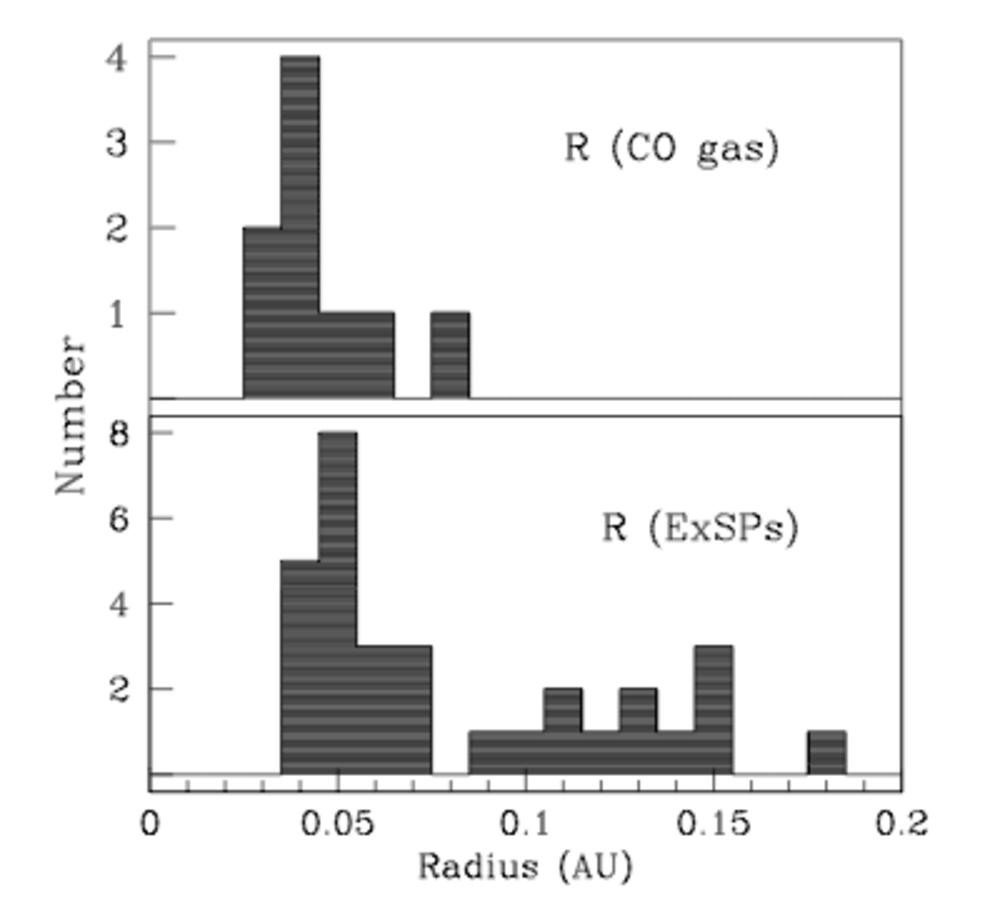
\includegraphics[width=\linewidth]{diskradius_najita07}
\caption[Inner disk radii from CO line emission]{
\label{fig:diskradius_najita07}
The top panel shows inner truncation radii of disks as inferred from the maximum velocity of CO vibrational emission. For comparison, the bottom panel shows the radial distribution of the hot Jupiter expolanets known at the time \citep{najita07a}.
}
\end{figure}

For the sub-mm and radio, detections have mostly involved CO and its isotopologues. The main advantage of this data, as opposed to the dust continuum, is that we obtain kinematic information. This can then be used to determine whether the (usually) poorly-resolved objects we see in the continuum have a velocity structure consistent with Keplerian rotation.  Figure \ref{fig:diskvel_tobin12} shows an example. Note that higher velocity emission tends to come from closer to the star, exactly as would be expected for a Keplerian disk. Indeed, when one fits the data to Keplerian rotation curves, they are entirely consistent. The number of sources for which this analysis has been done is not large, but it is growing.

\begin{figure}
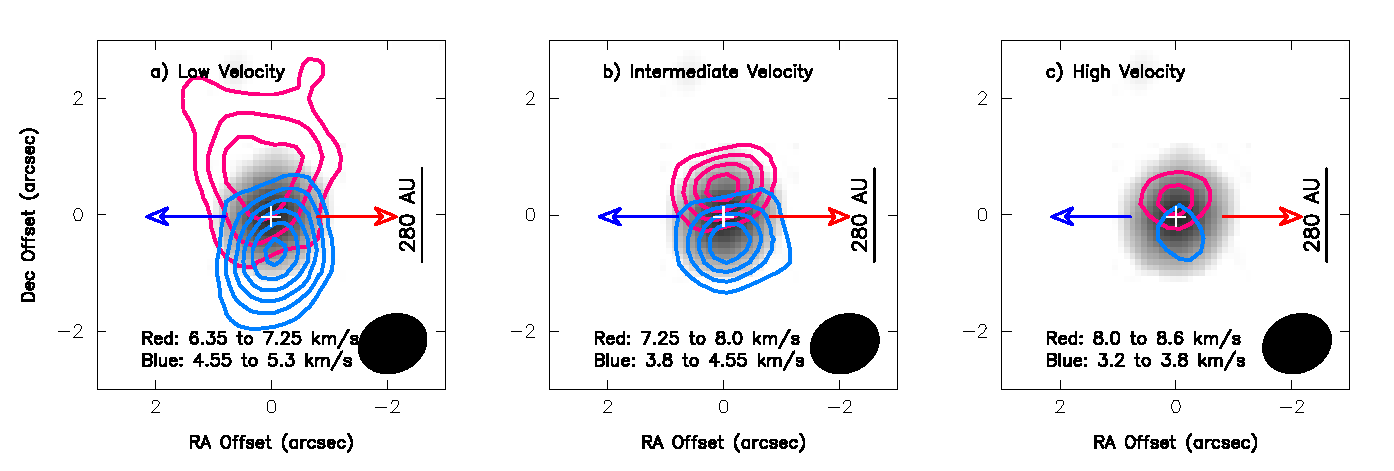
\includegraphics[width=\linewidth]{diskvel_tobin12}
\caption[$^{13}$CO channel maps of the disk in L1527]{
\label{fig:diskvel_tobin12}
Observed $^{13}$CO line emission from the disk in the core L1527. In each panel, grayscale shows dust continuum emission, white plus signs mark the location of the star, and the red and blue contours show the emission observed in the indicated velocity range. Black ovals show the observational beam, and red and blue arrows show the axis defined by an observed molecular outflow \citep{tobin12a}.
}
\end{figure}



\section{Observations of Outflows}

\subsection{Outflows in the Optical}

In addition to observing the disks themselves, we can observe the outflows that they drive. Outflows were first noticed in the 1950s based on optical observations by Herbig and Haro, working independently. The class of objects they discovered are known as Herbig-Haro, or HH, objects in their honor. HH objects were first seen as small patches of optical emission containing both continuum and a number of lines, most prominently H$\alpha$. The H$\alpha$ indicates the presence of ionization, but, unlike the large ionized regions generated by massive stars, where all species are highly ionized, HH objects also show signs of emission from neutral or weakly ionized species such as O~\textsc{i} and N~\textsc{ii}.

The standard interpretation of this sort of ionization structure is that we are seeing a fast shock. The shocked material is ionized, producing H$\alpha$ emission as it recombines. Both upstream and downstream of the shock itself, however, there is neutral material that is warm, either because it has had a chance to recombine but not to cool (for the downstream gas) or because it has been pre-heated by radiation from the shock (for the upstream gas). This produces the neutral or weakly ionized emission lines.

More sensitive measurements in the 1970s revealed that the bright emission knots Herbig and Haro saw are in fact connected by linear structures that also emit in optical, just with lower surface brightness. We can also see bow shocks at the heads of jets, where the plough into dense molecular gas (Figure \ref{fig:hhjet}).

\begin{figure}
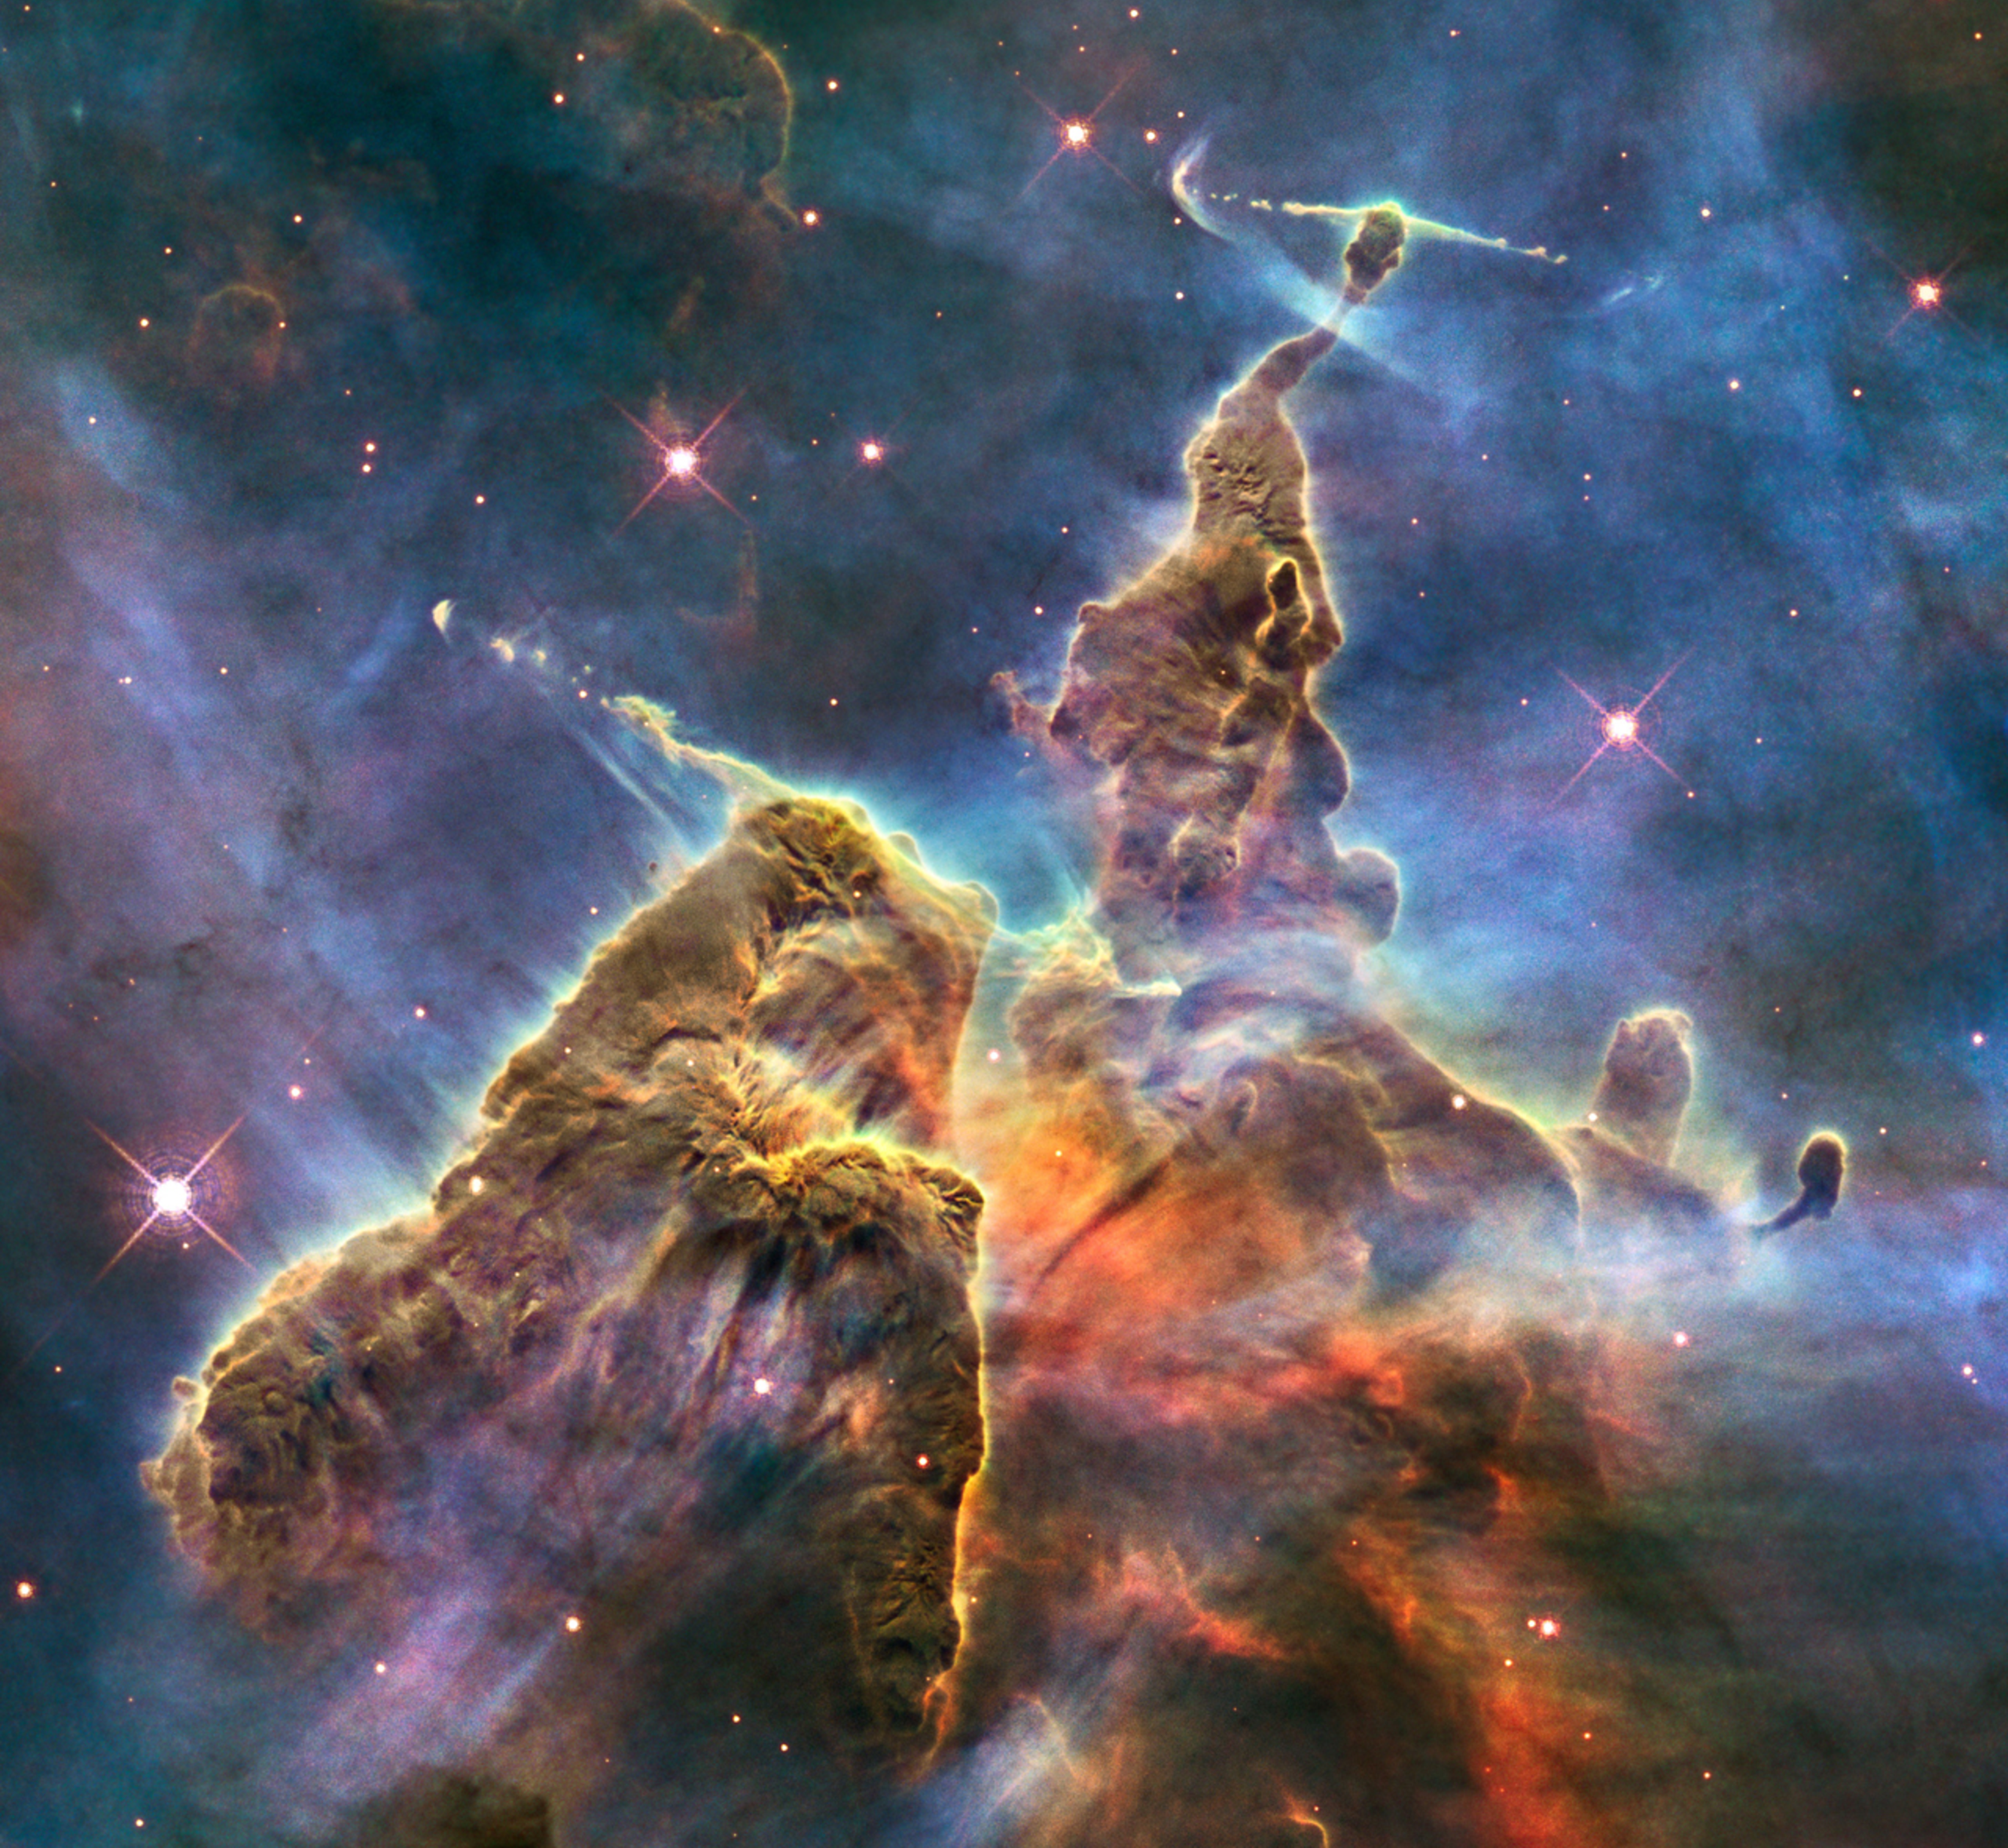
\includegraphics[width=\linewidth]{hhjet}
\caption[Herbig-Haro jets from \textit{HST}]{
\label{fig:hhjet}
Herbig-Haro jets imaged with the Hubble Space Telescope. Two jets are visible; one is at the tip of the ``pillar" near the top of the image, and another is near the edge of the structure in the middle-left part of the image. Bow shocks from the jets are clearly visible. Taken from \url{http://hubblesite.org/newscenter/archive/releases/2010/13/image/a/}.
}
\end{figure}

Today our interpretation of the HH knots is that they are locations where the jet has either encountered a dense region of interstellar material, producing a strong shock and bright emission, or where some variation in the velocity or mass flux being launched into the jet has caused an internal shock. The weaker emission in between the knots is caused by the interaction of the jet with a lower density environment. One can also detect this component in radio free-free emission, produced by electrons in the jet plasma.

The HH objects move fast enough to produce noticeable shifts in position and / or brightness over spans of $\sim 10$ years. The inferred velocities are typically hundreds of km s$^{-1}$. These velocities are also consistent with what we infer from Doppler shifts in cases where the jets is partly oriented toward us.

An important point is that these HH jets are usually bipolar, meaning that there is a clear driving star at the base of two HH objects propagating in opposite directions. Sometimes the knots of emission are even mirror symmetric, suggesting that they are produced by variations in the outflow velocity or mass flux originating at the point where the jet is launched.

Estimates of the density of the outflowing material based on models of the shocks suggest mass fluxes that range from $10^{-6}$ $\msun$ yr$^{-1}$ in class 0 sources, dropping to $10^{-8}-10^{-7}$ $\msun$ yr$^{-1}$ for classical T Tauri stars / class I sources. The inferred momentum flux is therefore of order $10^{-6}-10^{-3}$ $\msun$ km s$^{-1}$ yr$^{-1}$. These estimates are quite uncertainty however, since they are based on shock diagnostics, and tell us relatively little about the material in between the bright HH knots.


\subsection{Outflows in the Radio}

Optical and near-IR emission traces the regions where strong shocks heat the gas enough to excite transitions at these wavelengths. However, the jets of fast moving material only show the tip of the iceberg as far as the outflow is concerned. Observations in molecular lines reveal that narrow optical HH jets are accompanied by a much wider-angle, slower-moving, and more massive molecular outflow (Figure \ref{fig:molecular_outflow}).

\begin{figure}
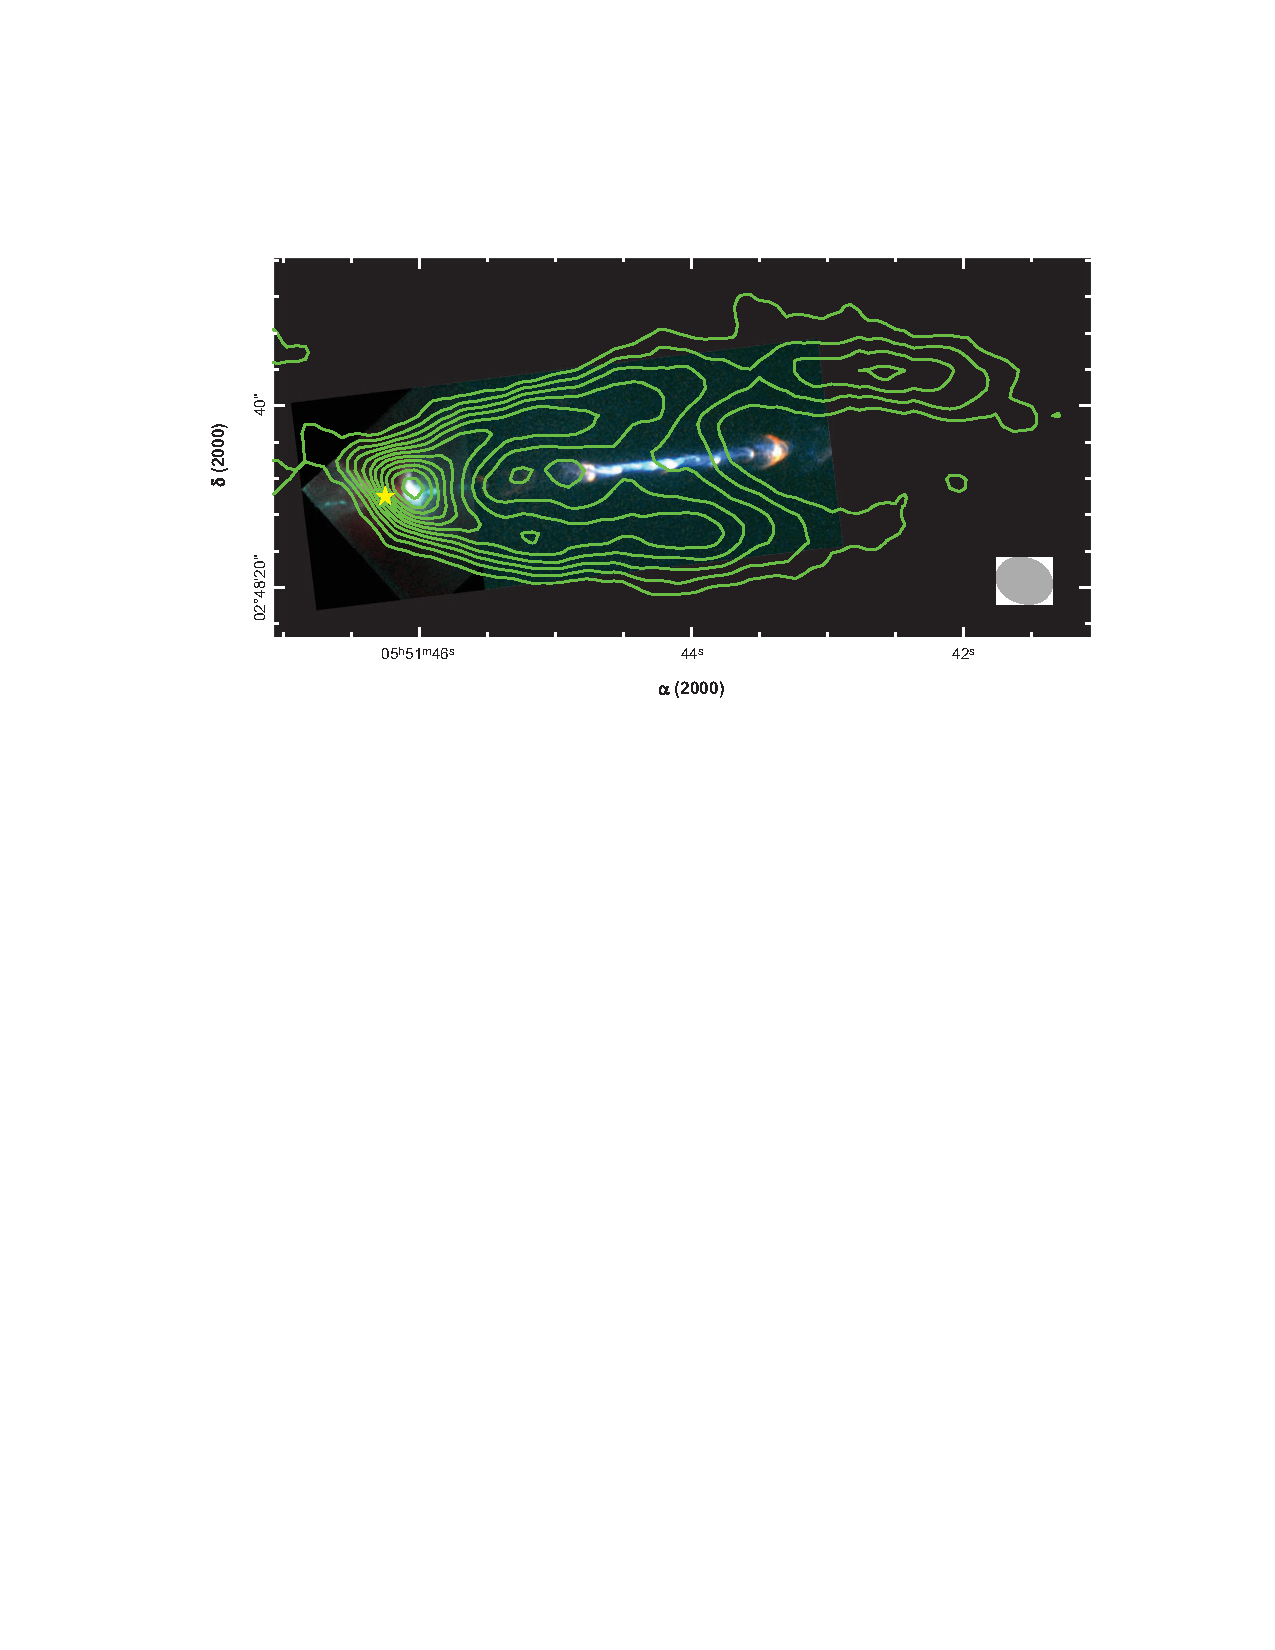
\includegraphics[width=\linewidth]{molecular_outflow}
\caption[A molecular outflow in HH111]{
Color shows an \textit{HST} image of the jet HH111. The green contours superimposed show an outflow detected as emission in the CO $J=1\rightarrow 0$ line at a velocity of 6 km s$^{-1}$ relative to the bulk of the material in the region. The yellow star marks the position of the driving source. The outflow is $\approx 0.2$ pc long. \citep{mckee07a}. 
}
\end{figure}

Molecular observations show large masses of molecular gas moving at $\sim 10$ km s$^{-1}$ -- the velocity is based on the Doppler shifts of the molecular lines used to observe the outflow. Again, we generally see a bipolar morphology. Depending on the outflow direction, this can consist of two lobes pointing in opposite directions on the sky, two lobes in the same position on the sky but with distinct red- and blue-shifted components, or some combination of the two.

Despite their lower velocities, these wind components actually contain the bulk of the outflow momentum, typically $10^{-4}-10^{-1}$ $\msun$ km s$^{-1}$ yr$^{-1}$, depending on the luminosity of the driving source. The molecular outflows are thought to consist primarily not of material ejected directly by the launching mechanism, but of ambient gas that has been swept up by this gas as it flows outward. The interaction is via shocks that can radiate, so energy is not conserved, but momentum is. This entrainment explains why the velocities of this material are so low compared to the material in the jets.

